\documentclass[12pt,a4paper]{article}
\usepackage[left=2cm,right=2cm,top=2cm,bottom=2cm]{geometry}
\usepackage[utf8]{inputenc}
\usepackage{amsmath}
\usepackage{amssymb}
\usepackage{graphicx}
\usepackage[english, russian]{babel}
\usepackage{indentfirst}
\usepackage{listings}
\usepackage{xcolor}
\usepackage{hyperref}
\usepackage{array}

\graphicspath{ {./plots/} }

\hypersetup{
    colorlinks=true,
    urlcolor= blue,
    citecolor=blue,
    linkcolor= blue,
}

\newcolumntype{P}[1]{>{\centering\arraybackslash}p{#1}}

\begin{document}

\begin{titlepage}

\Large

\begin{center}
Санкт-Петербургский \\ Политехнический университет Петра Великого

\vspace{10em}

Отчет по курсовой работе\\
по дисциплине "Математическая статистика"\\
по теме "Оценки коэффициентов линейной регрессии"\\

\vspace{2em}

\end{center}

\vspace{6em}

\newbox{\lbox}
\savebox{\lbox}{\hbox{Марков Михаил Денисович}}
\newlength{\maxl}
\setlength{\maxl}{\wd\lbox}
\hfill\parbox{12cm}{
\hspace*{3cm}\hspace*{-5cm}Студенты:\hfill\hbox to\maxl{Скворцов Владимир Сергеевич\hfill}\\
\hspace*{3cm}\hspace*{-5cm}\hfill\hbox to\maxl{Горюнов Максим Юрьевич\hfill}\\
\hspace*{3cm}\hspace*{-5cm}\hfill\hbox to\maxl{Голузин Егор Константинович\hfill}\\
\hspace*{3cm}\hspace*{-5cm}Преподаватель:\hfill\hbox to\maxl{Баженов Александр Николаевич}\\
\\
\hspace*{3cm}\hspace*{-5cm}Группа:\hfill\hbox to\maxl{5030102/10201}\\
}

\vspace{\fill}

\begin{center}
Санкт-Петербург \\2024
\end{center}

\end{titlepage}

\tableofcontents

\newpage

\section{Постановка задачи}

На основе имеющихся данных о выходных значениях вольтметра, изменяющихся с течением времени, при известных входных значениях подаваемого напряжения необходимо получить оценку данной зависимости с использованием следующих методов:
\begin{enumerate}
    \item Метод наименьших квадратов.
    \item Метод наименьших модулей.
\end{enumerate}
Для исследования предоставлен шестой столбец данных. Ссылка на исходный материал: https://disk.yandex.ru/d/OAQgCulS6NfbOQ.
\section{Используемые теоретические понятия}
\subsection{Метод наименьших квадратов}
При оценивании параметров регрессионной модели используют различные
методы. Один из наиболее распрстранённых подходов заключается в
следующем: вводится мера (критерий) рассогласования отклика и
регрессионной функции, и оценки параметров регрессии определяются так,
чтобы сделать это рассогласование наименьшим. Достаточно простые
расчётные формулы для оценок получают при выборе критерия в виде суммы
квадратов отклонений значений отклика от значений регрессионной функции
(сумма квадратов остатков):

\begin{equation} \label{eq:lsm}
    Q(\beta_0, \beta_1) = \sum \limits_{i=1}^n \varepsilon_i^2 =
    \sum \limits_{i=1}^n (y_i - \beta_0 - \beta_1 x_i)^2 \rightarrow
    \min_{\beta_0, \beta_1}.
\end{equation}

Задача минимизации квадратичного критерия \eqref{eq:lsm} носит название
задачи метода наименьших квадратов (МНК), а оценки \( \beta_0 \),
\( \beta_1 \) параметров \( \beta_0 \), \( \beta_1 \), реализующие минимум
критерия \eqref{eq:lsm}, называют МНК-оценками.

\subsection{Метод наименьших модулей}

Робастность оценок коэффициентов линейной регрессии (т.е. их
устойчивость по отношению к наличию в данных редких, но больших по
величине выбросов) может быть обеспечена различными способами. Одним из
них является использование метода наименьших модулей вместо метода
наименьших квадратов:

\begin{equation} \label{eq:lam}
    \sum \limits_{i=1}^n |y_i - \beta_0 - \beta_1 x_i| \rightarrow
    \min_{\beta_0, \beta_1}.
\end{equation}


\subsection{Бокс-плот Тьюки}
Боксплот (англ. box plot) — график, использующихся в описательной статистике, компактно изобрадающий одномерное распределение вероятностей. Такой вид диаграммы в удобной форме показывает медиану, нижний и верхний квартили и выбросы. Границами ящика служат первый и третий квартили, линия в середине ящика — медиана. Концы усов — края статистически значимой выборки (без выброса). Длину <<усов>> определяют разность первого квартиля и полутора межквартальных расстояний и сумма третьего квартиля и полутора межквартальных расстояний. Формула имеет вид

\begin{equation} \label{eq:box_plot}
X_1 = Q_1 - \frac{3}{2}(Q_3 - Q_1), \ X_2 = Q_3 + \frac{3}{2}(Q_3 - Q_1),
\end{equation}

где $X_1$ — нижняя граница уса, $X_2$ — верхняя граница уса, $Q_1$ — первый квартиль, $Q_3$ - третий квартиль.
Данные, выходящие за границы усов (выбросы), отображаются на графике в виде маленьких кружков.
Выбросами считаются величины $х$, такие что:

\begin{equation} \label{eq:outlier}
\left[
  \begin{array}{ll}
      x < X_1^T \\
      x > X_2^T
  \end{array}
\right .
\end{equation}\\\\
\section{Описание работы}
Лабораторные работы выполнены с использованием Python и сторонних
библиотек \verb!numpy!, \verb!pandas!, \verb!matplotlib!, \verb!seaborn!. Для каждого значения напряжения данные были обработаны при помощи боксплота Тьюки, для обработанных данных также был построен график исследуемой зависимости.

Ссылка на GitHub репозиторий:\\
\href{https://github.com/eagerbeaver04/Mathematical-statistics/tree/master/lab3}
{https://github.com/vladimir-skvortsov/math-stats-course-work}
\clearpage
\section{Результаты}
\subsection{Напряжение $U = -0.45V$}
\begin{figure}[htbp!]
    \begin{center}
        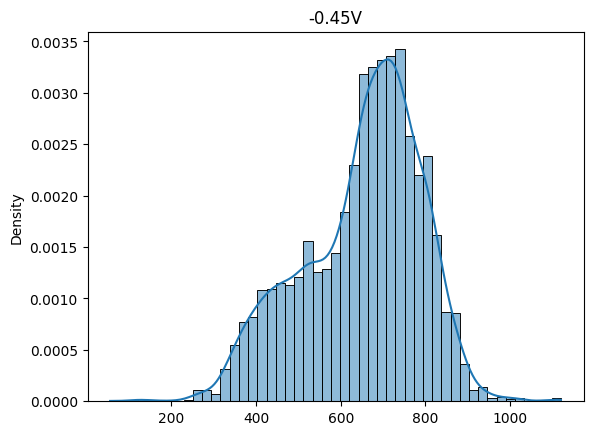
\includegraphics[width = 0.7\linewidth]{plots/-0.45Vhist.png}
        \caption{Гистограмма распределения значений выходного напряжения}
    \end{center}
\end{figure}
\begin{figure}[htbp!]
    \begin{center}
        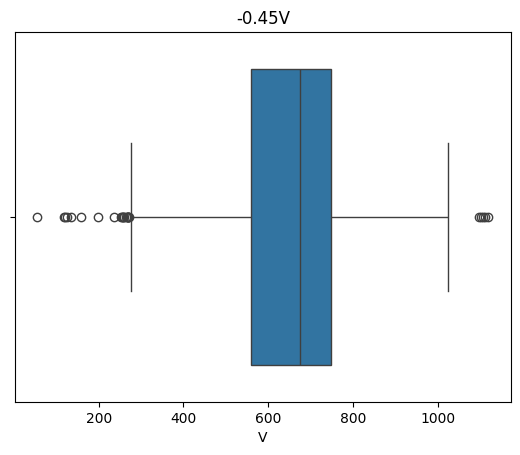
\includegraphics[width = 0.7\linewidth]{plots/-0.45Vbox.png}
        \caption{Боксплот распределения значений выходного напряжения}
    \end{center}
\end{figure}

\subsection{Напряжение $U = -0.35V$}
\begin{figure}[htbp!]
    \begin{center}
        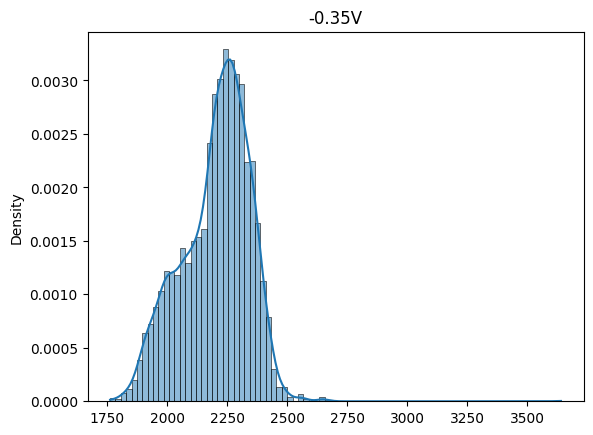
\includegraphics[width = 0.7\linewidth]{plots/-0.35Vhist.png}
        \caption{Гистограмма распределения значений выходного напряжения}
    \end{center}
\end{figure}
\begin{figure}[htbp!]
    \begin{center}
        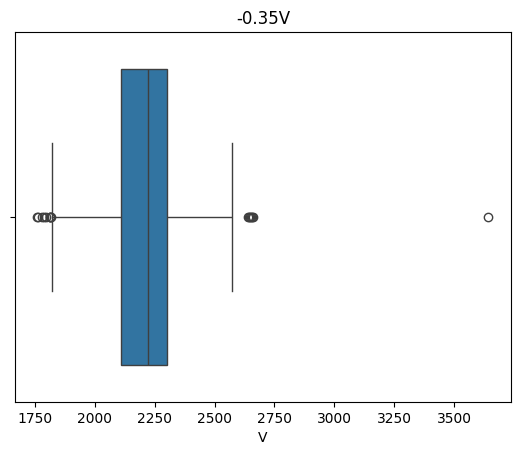
\includegraphics[width = 0.7\linewidth]{plots/-0.35Vbox.png}
        \caption{Боксплот распределения значений выходного напряжения}
    \end{center}
\end{figure}

\subsection{Напряжение $U = -0.25V$}
\begin{figure}[htbp!]
    \begin{center}
        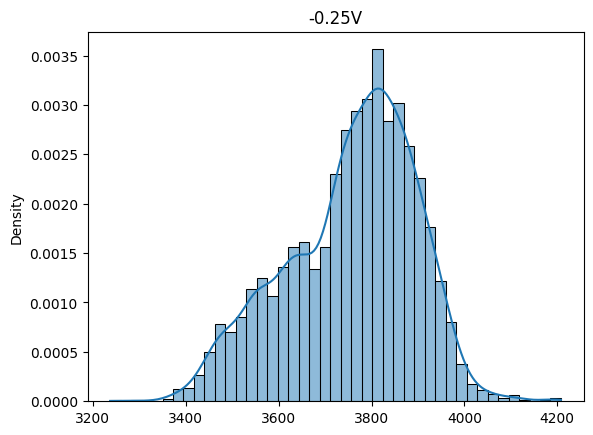
\includegraphics[width = 0.7\linewidth]{plots/-0.25Vhist.png}
        \caption{Гистограмма распределения значений выходного напряжения}
    \end{center}
\end{figure}
\begin{figure}[htbp!]
    \begin{center}
        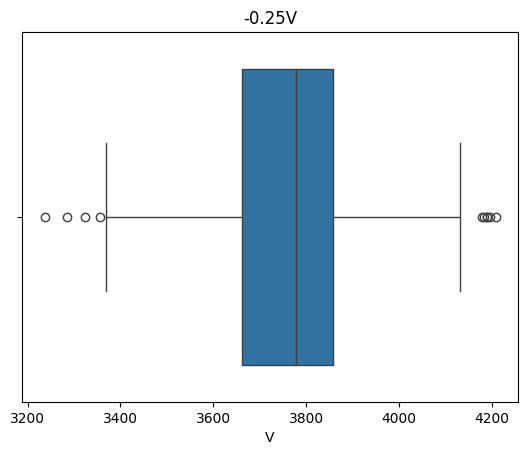
\includegraphics[width = 0.7\linewidth]{plots/-0.25Vbox.png}
        \caption{Боксплот распределения значений выходного напряжения}
    \end{center}
\end{figure}

\subsection{Напряжение $U = -0.15V$}
\begin{figure}[htbp!]
    \begin{center}
        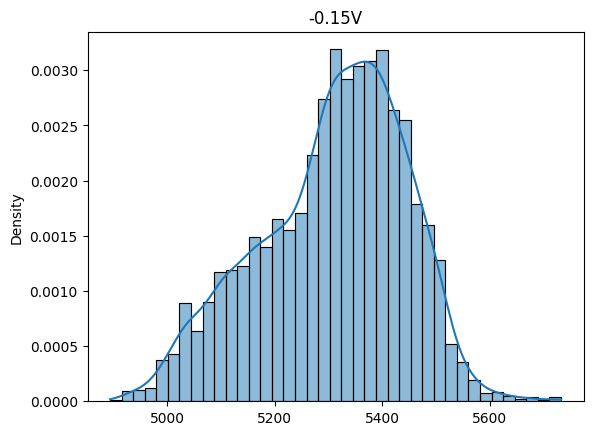
\includegraphics[width = 0.7\linewidth]{plots/-0.15Vhist.png}
        \caption{Гистограмма распределения значений выходного напряжения}
    \end{center}
\end{figure}
\begin{figure}[htbp!]
    \begin{center}
        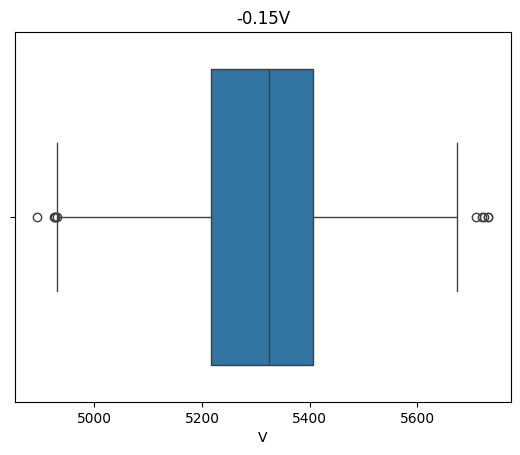
\includegraphics[width = 0.7\linewidth]{plots/-0.15Vbox.png}
        \caption{Боксплот распределения значений выходного напряжения}
    \end{center}
\end{figure}

\subsection{Напряжение $U = -0.05V$}
\begin{figure}[htbp!]
    \begin{center}
        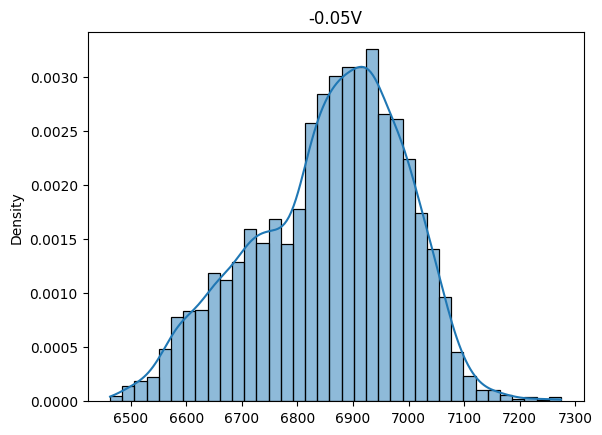
\includegraphics[width = 0.7\linewidth]{plots/-0.05Vhist.png}
        \caption{Гистограмма распределения значений выходного напряжения}
    \end{center}
\end{figure}
\begin{figure}[htbp!]
    \begin{center}
        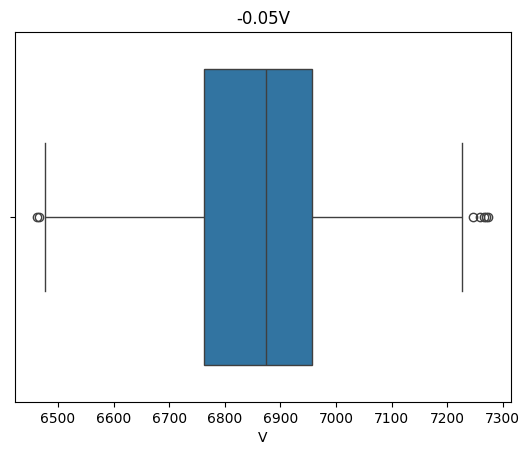
\includegraphics[width = 0.7\linewidth]{plots/-0.05Vbox.png}
        \caption{Боксплот распределения значений выходного напряжения}
    \end{center}
\end{figure}

\subsection{Напряжение $U = 0.0V$}
\begin{figure}[htbp!]
    \begin{center}
        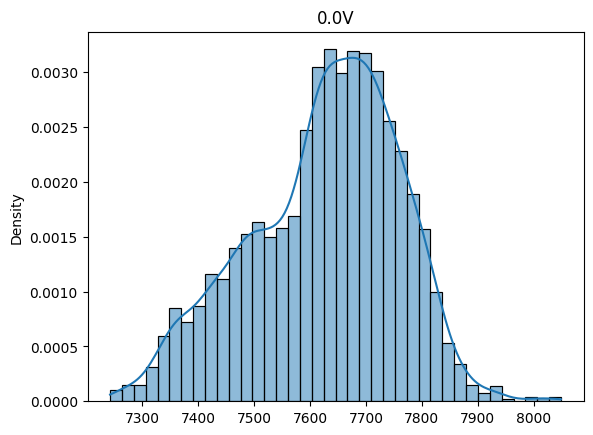
\includegraphics[width = 0.7\linewidth]{plots/0.0Vhist.png}
        \caption{Гистограмма распределения значений выходного напряжения}
    \end{center}
\end{figure}
\begin{figure}[htbp!]
    \begin{center}
        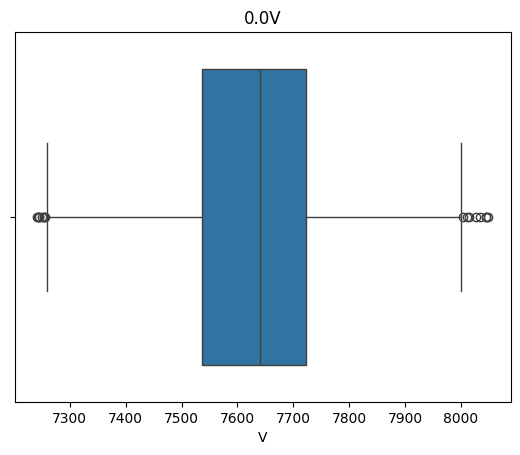
\includegraphics[width = 0.7\linewidth]{plots/0.0Vbox.png}
        \caption{Боксплот распределения значений выходного напряжения}
    \end{center}
\end{figure}

\subsection{Напряжение $U = 0.05V$}
\begin{figure}[htbp!]
    \begin{center}
        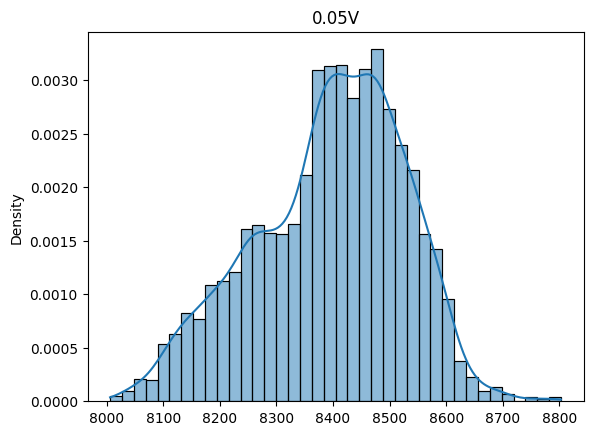
\includegraphics[width = 0.7\linewidth]{plots/0.05Vhist.png}
        \caption{Гистограмма распределения значений выходного напряжения}
    \end{center}
\end{figure}
\begin{figure}[htbp!]
    \begin{center}
        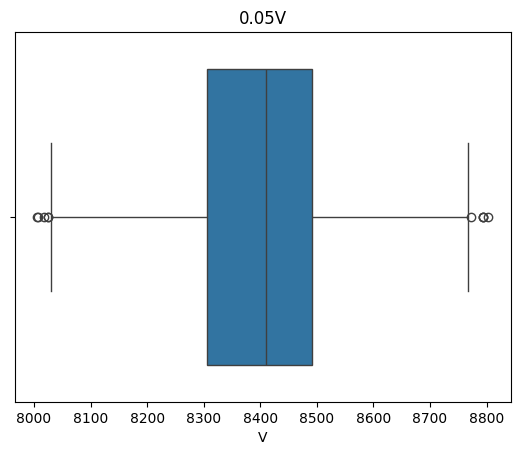
\includegraphics[width = 0.7\linewidth]{plots/0.05Vbox.png}
        \caption{Боксплот распределения значений выходного напряжения}
    \end{center}
\end{figure}

\subsection{Напряжение $U = 0.15V$}
\begin{figure}[htbp!]
    \begin{center}
        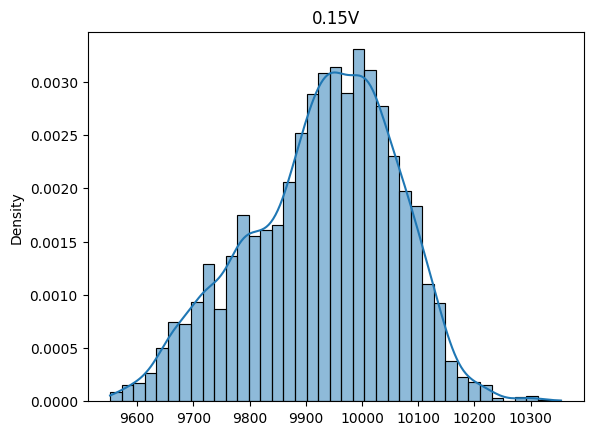
\includegraphics[width = 0.7\linewidth]{plots/0.15Vhist.png}
        \caption{Гистограмма распределения значений выходного напряжения}
    \end{center}
\end{figure}
\begin{figure}[htbp!]
    \begin{center}
        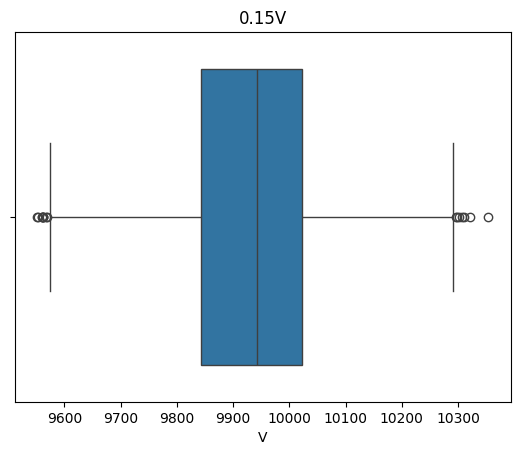
\includegraphics[width = 0.7\linewidth]{plots/0.15Vbox.png}
        \caption{Боксплот распределения значений выходного напряжения}
    \end{center}
\end{figure}

\subsection{Напряжение $U = 0.25V$}
\begin{figure}[htbp!]
    \begin{center}
        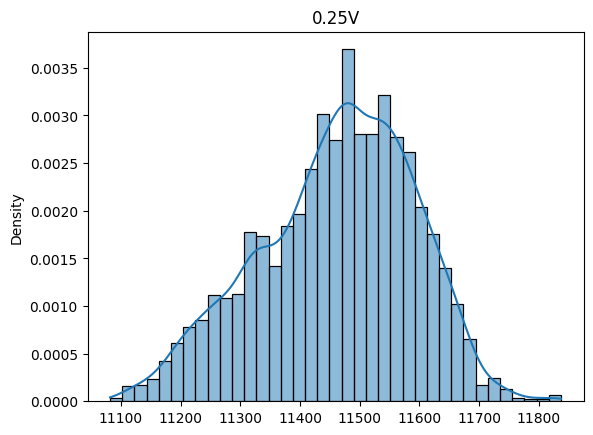
\includegraphics[width = 0.7\linewidth]{plots/0.25Vhist.png}
        \caption{Гистограмма распределения значений выходного напряжения}
    \end{center}
\end{figure}
\begin{figure}[htbp!]
    \begin{center}
        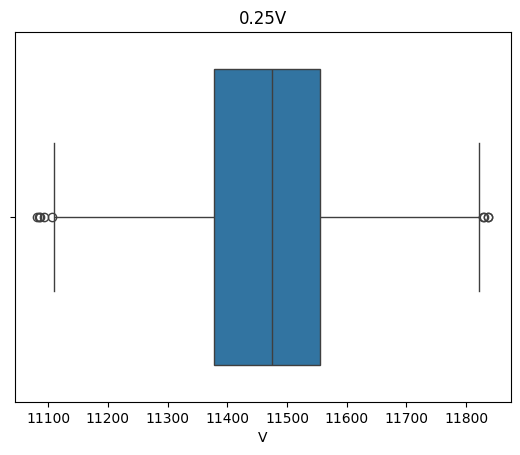
\includegraphics[width = 0.7\linewidth]{plots/0.25Vbox.png}
        \caption{Боксплот распределения значений выходного напряжения}
    \end{center}
\end{figure}

\subsection{Напряжение $U = 0.35V$}
\begin{figure}[htbp!]
    \begin{center}
        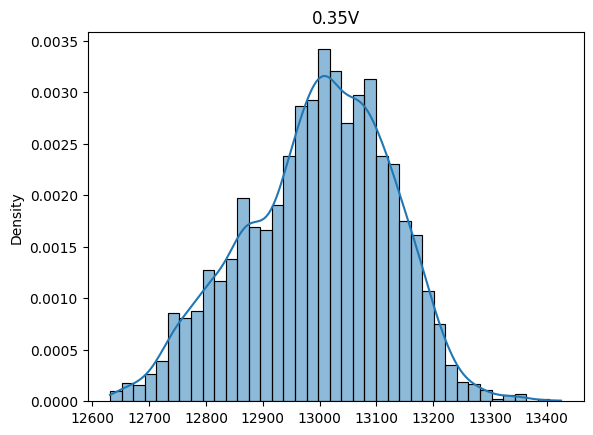
\includegraphics[width = 0.7\linewidth]{plots/0.35Vhist.png}
        \caption{Гистограмма распределения значений выходного напряжения}
    \end{center}
\end{figure}
\begin{figure}[htbp!]
    \begin{center}
        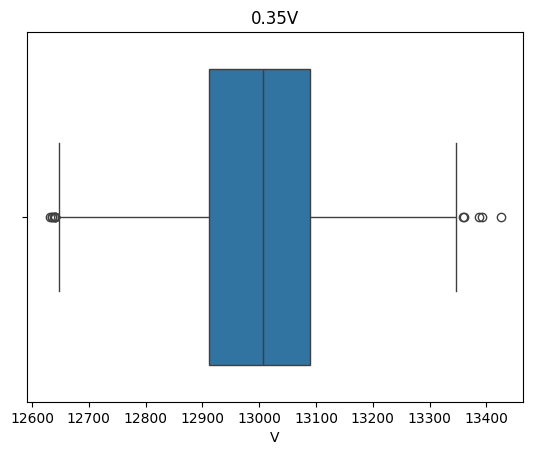
\includegraphics[width = 0.7\linewidth]{plots/0.35Vbox.png}
        \caption{Боксплот распределения значений выходного напряжения}
    \end{center}
\end{figure}

\subsection{Напряжение $U = 0.45V$}
\begin{figure}[htbp!]
    \begin{center}
        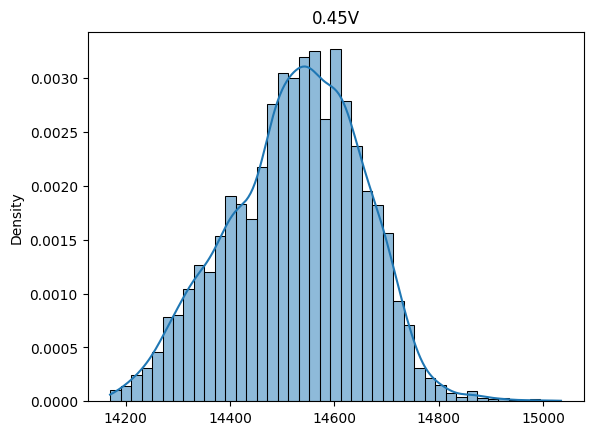
\includegraphics[width = 0.7\linewidth]{plots/0.45Vhist.png}
        \caption{Гистограмма распределения значений выходного напряжения}
    \end{center}
\end{figure}
\begin{figure}[htbp!]
    \begin{center}
        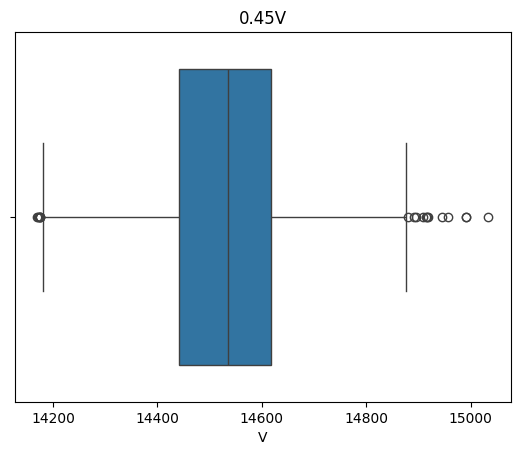
\includegraphics[width = 0.7\linewidth]{plots/0.45Vbox.png}
        \caption{Боксплот распределения значений выходного напряжения}
    \end{center}
\end{figure}

\begin{table}[htbp]
    \centering
    \begin{tabular}{ |c|c|c|c| }
        \hline
        -0.05 & 190.0 & 4931.0 & 5691.0 \\
        \hline
        -0.45 & 190.0 & 4931.0 & 5691.0 \\
        \hline
        -0.35 & 190.0 & 4931.0 & 5691.0 \\
        \hline
        0.35 & 190.0 & 4931.0 & 5691.0 \\
        \hline
        -0.25 & 190.0 & 4931.0 & 5691.0 \\
        \hline
        0.05 & 190.0 & 4931.0 & 5691.0 \\
        \hline
        0.15 & 190.0 & 4931.0 & 5691.0 \\
        \hline
        0.45 & 190.0 & 4931.0 & 5691.0 \\
        \hline
        0.0 & 190.0 & 4931.0 & 5691.0 \\
        \hline
        0.25 & 190.0 & 4931.0 & 5691.0 \\
        \hline
        -0.15 & 190.0 & 4931.0 & 5691.0 \\
        \hline
    \end{tabular}
    \caption{Боксплот Тьюки}
\end{table}

\subsection{Линейная регрессия до предобработки данных}
\subsection{Напряжение $U = 0.05V$}
\begin{figure}[htbp!]
    \begin{center}
        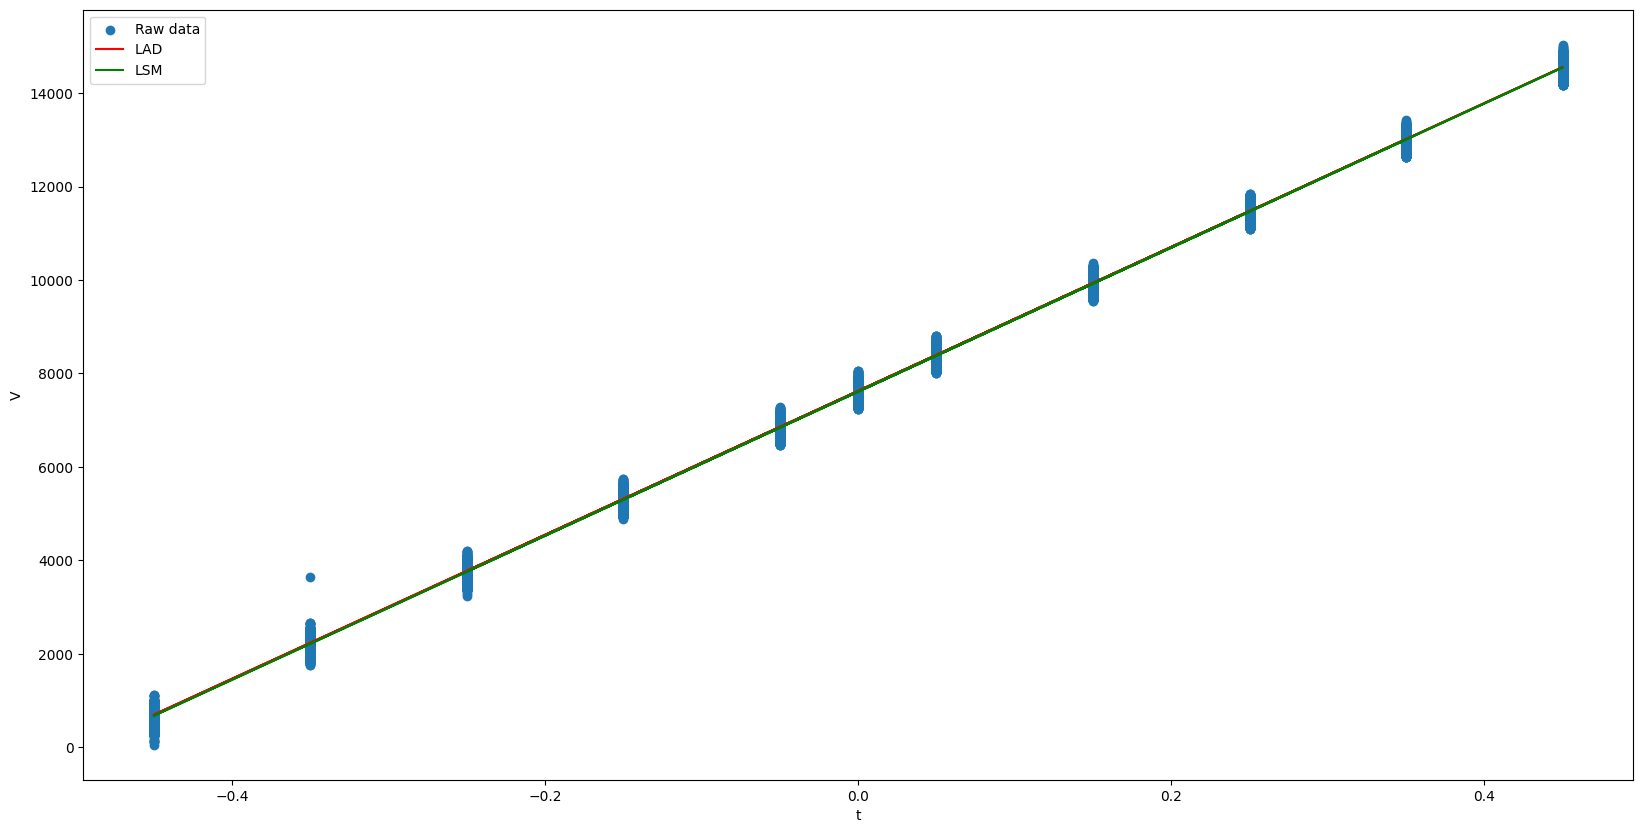
\includegraphics[width = 0.7\linewidth]{plots/unfiltered.png}
        \caption{Полученные прямые для необработанных данных}
    \end{center}
\end{figure}

\subsection{Линейная регрессия после предобработки данных}
\subsection{Напряжение $U = 0.05V$}
\begin{figure}[htbp!]
    \begin{center}
        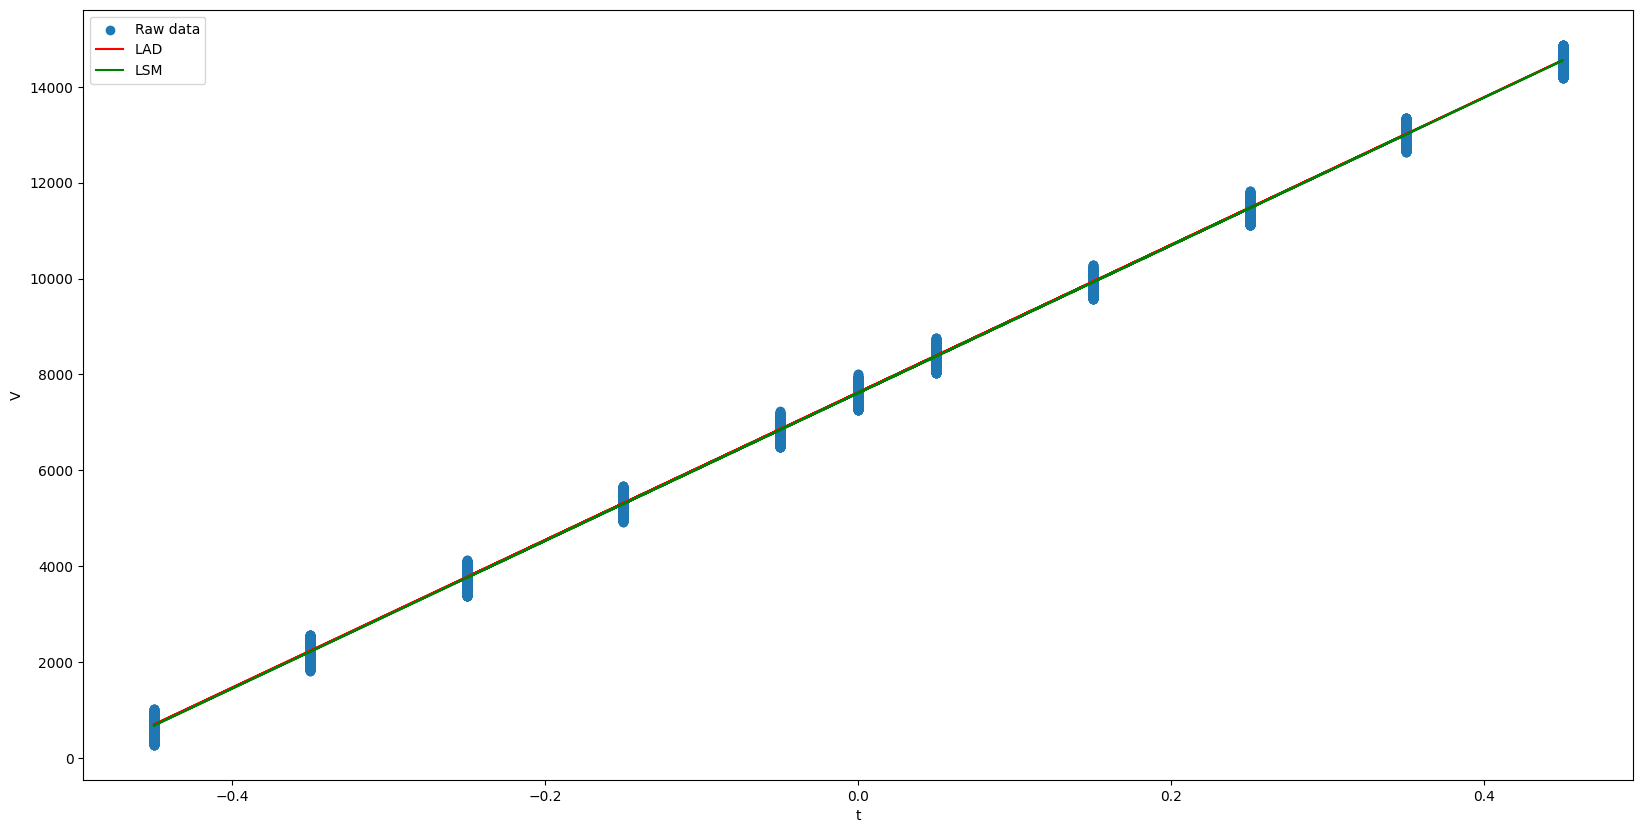
\includegraphics[width = 0.7\linewidth]{plots/filtered.png}
        \caption{Полученные прямые для обработанных данных}
    \end{center}
\end{figure}

\newpage

\section{Выводы}

\begin{enumerate}
    \item Метод наименьших квадратов позволяет при помощи нетрудоемких вычислений получить коэффициенты линейной регрессии зависимых величин.
    \item Метод наименьших модулей обеспечивает робастность оценок коэффициентов линейной регрессии.
    \item При этом предобработка данных позволяет более точно оценить параметры линейной регрессии. Так, при использовании предобработки из исследуемых данных удаляются выбросы, которые понижают точность полученных без предобработки результатов.
\end{enumerate}

\newpage

\end{document}
